\documentclass[11pt,a4paper]{ivoa}
\input tthdefs

\usepackage{xspace}
% Standard terms used throughout the document,
% defined as macro commands to maintain consistency

% Using non-breaking space character.
% https://stackoverflow.com/a/1012891

\newcommand{\xml} {XML}
\newcommand{\json} {JSON}
\newcommand{\yaml} {YAML}

\newcommand{\datamodel} {data~model}
\newcommand{\webservice} {webservice}
\newcommand{\webbrowser} {web browser}

\newcommand{\ivoa} {IVOA}
\newcommand{\uws} {UWS}
\newcommand{\vospace} {VOSpace}

\newcommand{\execplanner} {ExecutionPlanner}
\newcommand{\execworker} {ExecutionWorker}
\newcommand{\executionplanner} {Execution~Planner}
\newcommand{\executionplanning} {Execution~Planning}

\newcommand{\jupyter} {Jupyter}
\newcommand{\jupyterhub} {JupyterHub}
\newcommand{\binderhub} {BinderHub}
\newcommand{\jupyternotebook} {Jupyter notebook}

\newcommand{\esap} {ESAP}
\newcommand{\escape} {ESCAPE}
\newcommand{\datalake} {DataLake}
\newcommand{\rucio} {Rucio}

\newcommand{\python} {Python}

\newcommand{\apache} {Apache}
\newcommand{\spark} {Spark}
\newcommand{\pyspark} {PySpark}
\newcommand{\zeppelin} {Zeppelin}

\newcommand{\ocicontainer} {OCI~container}
\newcommand{\docker} {Docker}
\newcommand{\dockercompose} {Docker compose}
\newcommand{\dockercontainer} {Docker container}

\newcommand{\openstack} {Openstack}
\newcommand{\kubernetes} {Kubernetes}

\newcommand{\codeword}[1] {\texttt{#1}}
\newcommand{\footurl}[1] {\footnote{\url{#1}}}

\newcommand{\dataset} {dataset}
\newcommand{\datascience} {data~science}
\newcommand{\scienceplatform} {science~platform}

\newcommand{\executable} {\textit{executable}}
\newcommand{\executablething} {\textit{executable}~thing}
\newcommand{\excutabletask} {\textit{executable} task}
\newcommand{\workerjob} {\textit{job}}

\newcommand{\cpu} {CPU}
\newcommand{\gpu} {GPU}
\newcommand{\nvidiagpu} {NVIDIA~AD104~GPU}

\newcommand{\job} {\textit{job}}
\newcommand{\task} {task}

\newcommand{\scalable} {scalable}

\usepackage{listings}
\usepackage{xcolor}

%\colorlet{punct}{red!60!black}
\colorlet{numb}{magenta!60!black}
\definecolor{html-gray}{HTML}{EEEEEE}
\definecolor{light-gray}{gray}{0.95}
\definecolor{delim}{RGB}{20,105,176}

\lstset{
    basicstyle=\small\ttfamily,
    columns=fullflexible,
    frame=none,
    backgroundcolor=\color{light-gray},
    stepnumber=1,
    %numbers=left,
    numbers=none,
    numberstyle=\small,
    numbersep=8pt,
    %xleftmargin=\parindent,
    xrightmargin=1cm,
    showstringspaces=false,
    keepspaces=true,
    breaklines=true,
    linewidth=14cm,
    frame=none
}

% https://tex.stackexchange.com/questions/83085/how-to-improve-listings-display-of-json-files
% https://tex.stackexchange.com/a/83100
% https://tex.stackexchange.com/questions/10828/indent-a-code-listing-in-latex
% https://tex.stackexchange.com/a/10831
\lstdefinelanguage{json}{
    literate=
     *{0}{{{\color{numb}0}}}{1}
      {1}{{{\color{numb}1}}}{1}
      {2}{{{\color{numb}2}}}{1}
      {3}{{{\color{numb}3}}}{1}
      {4}{{{\color{numb}4}}}{1}
      {5}{{{\color{numb}5}}}{1}
      {6}{{{\color{numb}6}}}{1}
      {7}{{{\color{numb}7}}}{1}
      {8}{{{\color{numb}8}}}{1}
      }

\lstdefinelanguage{yaml}{
    literate=
     *{0}{{{\color{numb}0}}}{1}
      {1}{{{\color{numb}1}}}{1}
      {2}{{{\color{numb}2}}}{1}
      {3}{{{\color{numb}3}}}{1}
      {4}{{{\color{numb}4}}}{1}
      {5}{{{\color{numb}5}}}{1}
      {6}{{{\color{numb}6}}}{1}
      {7}{{{\color{numb}7}}}{1}
      {8}{{{\color{numb}8}}}{1}
      }

\hyphenation{Exe-cut-able-Thing}

\title{IVOA Execution Planner}

% see ivoatexDoc for what group names to use here; use \ivoagroup[IG] for
% interest groups.
\ivoagroup{GWS}

\author[http://www.ivoa.net/twiki/bin/view/IVOA/DaveMorris]
       {Dave Morris}

\editor[http://www.ivoa.net/twiki/bin/view/IVOA/DaveMorris]
       {Dave Morris}

% \previousversion[????URL????]{????Concise Document Label????}
\previousversion{This is the first public release}

\begin{document}
\begin{abstract}
\label{abstract}

One of the long term goals of the IVOA has been to enable users to
move the code to the data.
This is becoming more and more important as the size and complexity
of the \dataset{}s available in the virtual observatory increases.
%\citep{gaia-at-esac}
%\footurl{https://www.skao.int/en/explore/big-data}
%\footurl{https://www.lsst.org/scientists/keynumbers}

The \ivoa{} \executionplanner{} provides a step towards making this possible.

The \ivoa{} \executionplanner{} is designed to address a specific question;
given an executable thing, e.g. a \python{} program or \jupyternotebook{}.
What facilities are available to run it?

To do this, the \ivoa{} \executionplanner{} specification defines
a \datamodel{} and \webservice{} API for describing executable things
and the resources needed to execute them.

Together these components enable a user to ask a simple question
\textit{"Where (and when) can I execute my program?"}

This in turn enables users to move code between \scienceplatform{}s.
Allowing them to develop their code on one platform and then apply it to a different
\dataset{} by sending it to execute on another platform.

\end{abstract}

\section*{Acknowledgments}
\label{acknowledgments}

The authors would like to thank all the participants in the IVOA and ESCAPE projects
who have contributed their ideas, critical reviews, and suggestions to this document.

\section*{Conformance-related definitions}

The words ``MUST'', ``SHALL'', ``SHOULD'', ``MAY'', ``RECOMMENDED'', and
``OPTIONAL'' (in upper or lower case) used in this document are to be
interpreted as described in IETF standard RFC2119 \citep{std:RFC2119}.

The \emph{Virtual Observatory (VO)} is a general term for a collection of
federated resources that can be used to conduct astronomical research,
education, and outreach.
The \href{https://www.ivoa.net}{International Virtual Observatory Alliance (IVOA)}
is a global collaboration of separately funded projects to develop standards and
infrastructure that enable VO applications.

\section{Introduction}
\label{introduction}

The \ivoa{} \executionplanner{} specification defines two \webservice{} interfaces,
the \execplanner{} and the \execworker{}, and a common \datamodel{} for describing
executable tasks.

Together these provide a common interface for service discovery, resource allocation
and execution scheduling across a heterogeneous federation of different types of
execution platform.

\begin{itemize}
    \item \execplanner{} \webservice{} – a discovery service to find execution platforms, allocate resources and schedule execution.
    \item \execworker{} \webservice{} – an asynchronous service for executing tasks (based on the \ivoa{} \uws{} pattern).
    \item \execplanner{} \datamodel{} – a common data model for describing an executable thing and its resource requirements.
\end{itemize}

\subsection{Role within the VO Architecture}
\label{subsec:ivoarole}

% As of ivoatex 1.2, the architecture diagram is generated by ivoatex in
% SVG; copy ivoatex/archdiag-full.xml to role_diagram.xml and throw out
% all lines not relevant to your standard.
% Notes don't generally need this.  If you don't copy role_diagram.xml,
% you must remove role_diagram.pdf from SOURCES in the Makefile.
\begin{figure}
\centering
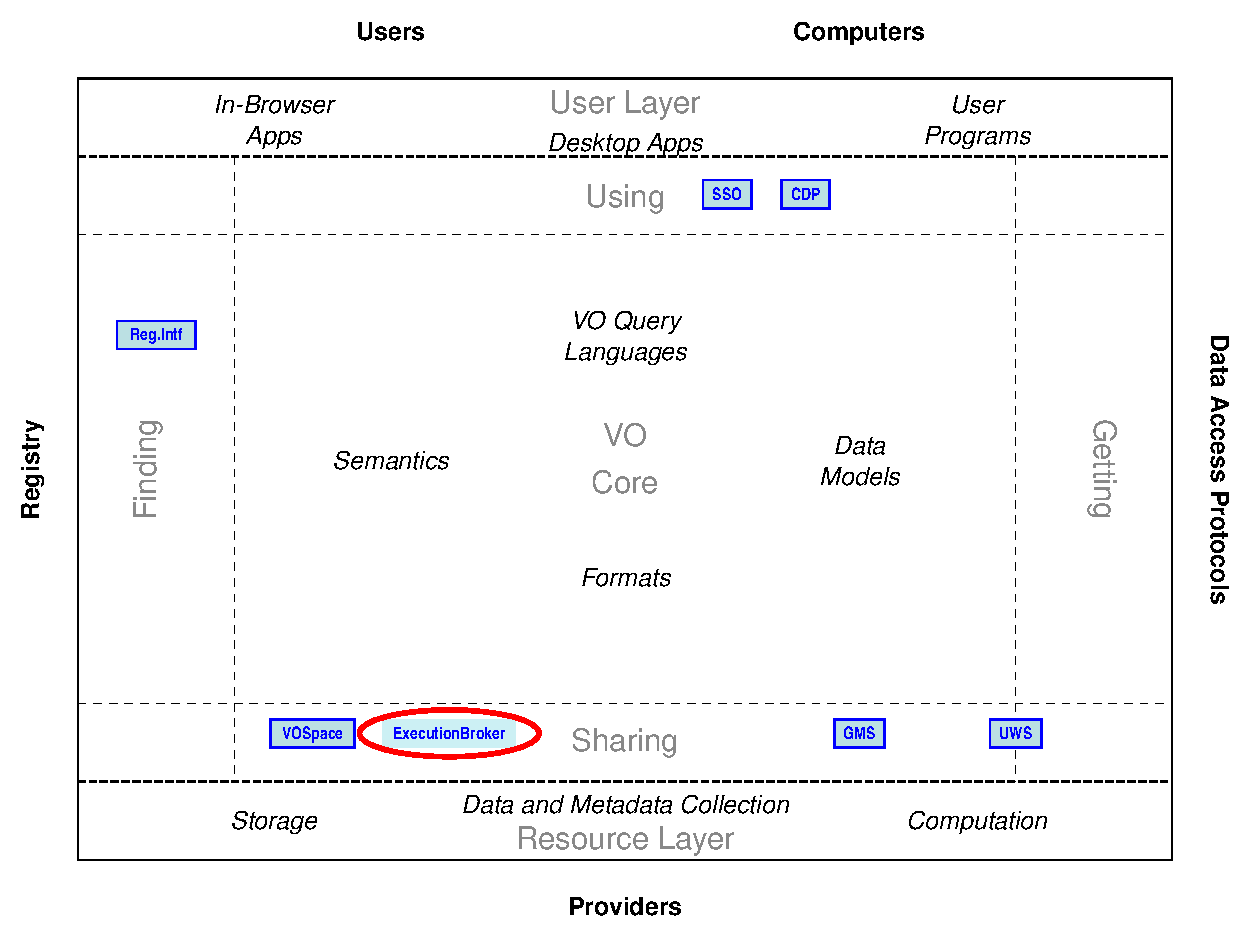
\includegraphics[width=0.9\textwidth]{role_diagram.pdf}
\caption{Architecture diagram showing the \ivoa{} \executionplanner{}'s role in the \ivoa}
\label{fig:archdiag}
\end{figure}

The IVOA Architecture\citep{2010ivoa.rept.1123A} provides a high-level view of how IVOA
standards work together to connect users and applications with providers of data
and services.
Fig.~\ref{fig:archdiag} shows the role the \ivoa{} \executionplanner{} plays within this architecture.

In response to the increasing size and complexity of the next generation of science \dataset{}s
a number of \ivoa{} members are developing intergrated \scienceplatform{}s which bring
together the \dataset{}s co-located with the compute resources needed to analyse
them.\footurl{https://data.lsst.cloud/}\footurl{https://rsp.lsst.io/index.html}

The \scienceplatform{}s make extensive use of the \ivoa{} data models and
vocabularies to describe their \dataset{}s, and use the \ivoa{} data access
services to find and access data from other data providers.
In addition, some of the \scienceplatform{}s use \ivoa{} \vospace{} services to manage
data transfers to and from local storage co-located with the compute resources.

However, to date the \ivoa{} does not provide any APIs or \webservice{} interfaces that
enable \scienceplatform{}s to exchange the software used to analyse the data.
The \ivoa{} \executionplanner{} provides a step towards making this possible.

This places the \ivoa{} \executionplanner{} in the same region of the \ivoa{} architecture
as the \ivoa{} \vospace{} specification \citep{2009ivoa.specQ1007G},
providing an infrastructure level service that enables service discovery,
resource allocation and execution scheduling across a heterogeneous federation
of execution platforms.

The \ivoa{} \executionplanner{} specification refers to the
\ivoa{} Single-Sign-On standard \citep{2017ivoa.spec.0524T}
for authentication (see section xx )%\ref{subsec:authentication}
and the
\ivoa{} Credential Delegation Protocol \citep{2010ivoa.spec.0218P}
for delegating credentials to other services.

The \ivoa{} \executionplanner{} specification also describes how to register
an \execplanner{} service in the
\ivoa{} Registry \citep{2009ivoa.spec.1104B},
making it findable within the wider context of the VO.

\subsection{Executable things}
\label{executablething}

To understand the problem that the \ivoa{} \executionplanner{} is trying to solve
it is useful to describe what an \executablething{} is in this context.
In general terms, this document refers to something that can be executed, or run,
as an \executable.

To explain what this means we can start with a science domain function that we want to perform.
For example, the mathematical concept of the square root of a number.
We can calculate the square root of a positive number using the Newton–Raphson
algorithm\footurl{https://en.wikipedia.org/wiki/Newton\%27s_method}
which produces successively closer approximations to the result.
However, in general case, this mathematical description of the algorithm would not be
considered to be an \executablething.

We can write a \python{} program to use this algorithm to calculate the square root of a number.
This is the first identifiable \executablething{} in our example.
To be able to use this \executablething{}, you would need a computing resource with the appropriate
hardware and software environment. In this case, a computing resource with the \python{} interpreter
installed along with any additional \python{} modules required by the program.
This environment is often referred to as the \python{} runtime.

In the context of \scienceplatform{}s and \datascience{}, a common pattern is to provide this environment
using an OCI\footurl{https://opencontainers.org/},
or Docker\footurl{https://docs.docker.com/get-started/what-is-a-container/} container,
to package the \python{} program and runtime together as a single binary object.
This package, or container, is itself an \executablething{}. One which requires a different execution
environment than the original \python{} program.
The aim of containerization is to package \executablething{}s together with the software environment
they need as a binary object that interfaces with a standard execution environment,
referred to as the \textit{container runtime}.
To be able to use this \executablething{}, you would need a computing resource with the appropriate
hardware and software environment. In this case, a computing resource with the \ocicontainer{} runtime installed.

We could also create a \jupyternotebook{} that demonstrates how to use our \python{} program.
This is the third \executablething{} in our example.
One which provides an interactive environment for the user to experiment with.
As before, to be able to use this \executablething{}, we would need a computing resource with
the appropriate hardware and software environment.
In this case, a computer with the \jupyternotebook{} platform installed along with all the \python{} modules
needed by our \python{} program.
In the context of \scienceplatform{}s and \datascience{}, a common pattern is to provide this environment as a \webservice{}
that allows the user to connect to the \jupyternotebook{} via a \webbrowser.

From one algorithm that implements a science domain function, we have created three different \executablething{}s.
A \python{} program, an \ocicontainer{} packaging the \python{} program, and an interactive \jupyternotebook{}
that demonstrates how to use the \python{} program.
Each of which requires a different computing environment to execute.
A basic \python{} runtime, the \ocicontainer{} runtime, and a \jupyternotebook{} service.

We may also want to consider the data that we are applying the algorithm to.
If we are running some small experiments to learn how to use the algorithm, then a basic computing
resource will probably be sufficient.
However, if we have a \dataset{} of ten million numbers that we want to process, then we may
need to consider adding extra storage to handle the input data and the results.
For a large \dataset{} it may also be worth using a \gpu{} to accelerate the calculation steps
for such a large \dataset{}.

The \ivoa{} \executionplanner{} \datamodel{} provides a way to describe what each of these \executablething{}s
are and what resources are needed to execute them.
This can include things like number of \cpu{} cores and amount of memory it needs,
whether it needs a \gpu{}, the location of the input data, the storage space needed to perform
the calculation and the storage space needed to save the results.

\subsection{Type URIs and specifications}
\label{type-and-spec}

Several parts of the \ivoa{} \executionplanner{} \datamodel{} follow a common pattern, using a URI
to identify a \codeword{type} followed a \codeword{spec} section to fill in the details.
This pattern is adopted from a similar pattern used by \kubernetes{} to describe components
that are deployed using the control interface.

However, the \executionplanner{} \datamodel{} specifically recomends using a resolvable, long lasting,
URL as the type identifier.

The reasoning behind this is that if a service provider notices several clients are requesting
\textit{'encabulation'} on their compute nodes, the service provider may not know what this means.
However, if we use a resolvable URL to identify the type\footurl{https://tinyurl.com/encabulation},
a service provider can use it to find a human readable description and decide whether they want
to provide it on their platform.

To the \webservice{} software both of these requests are just a simple string comparison against a
dictionary of known terms:

\begin{lstlisting}[]
Request  - Can this platform provide 'encabulation' ?
Response - YES|NO
\end{lstlisting}

\begin{lstlisting}[]
Request  - Can this platform provide 'https://tinyurl.com/encabulation' ?
Response - YES|NO
\end{lstlisting}

The second form provides a mechanism for linking the type identifier to a human readable description.

\section{Client-server conversation}
\label{conversation}

The core idea behind the \ivoa{} \executionplanner{} is based on a conversation between a client
and one or more \execplanner{} services to discover where, how, and when, an \executablething{} can be
executed.

The conversation starts with the client sending a description of the \executablething{} they want to
run to the
\execplanner{} services, which respond with a top level \codeword{YES|NO} answer, and if
the answer is \codeword{YES}, a list of offers describing how it
can be executed on their platform.

\begin{lstlisting}[]
Request  - Can this platform execute <task> ?
Response - YES, list of <offer>[]
\end{lstlisting}

The client can then choose which of the offers it wants to use and reply
with a message accepting the offer.
In response the \execplanner{} will mark the resources in the offer as reserved,
initiate a \workerjob{} in an \execworker{} service to execute the task
and reply with details of how to access it.

\begin{lstlisting}[]
Request  - I accept <offer>[n]
Response - <job details>
\end{lstlisting}

The client can then uses the connection details in the \workerjob{} response to contact
the \execworker{} service and track its status.

Note that the client does not need to cancel the offers made by the other \execplanner{} services.
Offers are only valid for a limited period of time, and expire naturally when they reach the end
of their lifetime.

A good way of explaining how a client would use the \datamodel{} to describing the \executablething{}
is to consider a series of questions that a client would ask to discover if a platform has the
resources available to execute the task.

\subsection{The \executable{}}
\label{executable}

At the simplest level the client just needs to check whether a platform is able to execute a particular
type of \excutabletask{}.
For example, \textit{"Is this platform able to run a \jupyternotebook{}?"}

In order to do this, the request needs to specify the task type, e.g. \jupyternotebook{},
along with details about it, e.g. where to fetch the notebook from.

The information in this part of the \datamodel{} will be different for each type of \executable{}.
Rather than try to model every possible type of \executable{} in one large \datamodel{},
the \datamodel{} for each type is described in an extension to the core \datamodel{}.

To support this, the core \datamodel{} defines two fields:
\begin{itemize}
  \item \codeword{type} - a URI identifying the type of \executable{}.
  \item \codeword{spec} - a place holder for type specific details.
\end{itemize}

\begin{lstlisting}[]
# ExecutionPlanner client request.
# Details of the executable.
executable:

  # A URI identifying the type of executable.
  # e.g.
  # https://www.purl.org/ivoa.net/ep/task-type/oci-container
  # https://www.purl.org/ivoa.net/ep/task-type/jupyter-notebook
  type: "https://www.purl.org/ivoa.net/ep/task-type/example"

  # The details, specific to the type of executable.
  spec: {}
\end{lstlisting}

The \datamodel{} for each type of \executable{} defines the metadata needed to
describe that particular type.
For example, the \datamodel{} for a \jupyternotebook{} needs to describe where
to fetch the source code for the notebook from.
\begin{lstlisting}[]
# ExecutionPlanner client request.
# Details of the executable.
executable:
  # A URI identifying the type of executable.
  type: "https://www.purl.org/ivoa.net/ep/task-type/jupyter-notebook"

  # The details, specific to a Jupyter notebook.
  spec:
    notebook: "https://.../example.jpnb"
\end{lstlisting}

It may also include a reference to a \codeword{requirements.txt} file that describes any additional \python{}
libraries needed to run the notebook.
\begin{lstlisting}[]
# ExecutionPlanner client request.
# Details of the executable.
executable:
  # A URI identifying the type of executable.
  type: "https://www.purl.org/ivoa.net/ep/task-type/jupyter-notebook"

  # The details, specific to a Jupyter notebook.
  spec:
    notebook: "https://.../example.jpnb"
    requirements: "https://.../requirements.txt"
\end{lstlisting}

The \datamodel{} for an \ocicontainer{} needs to describe what operating system and system architecture
the container is built for, and where to fetch the binary image from.

\begin{lstlisting}[]
# ExecutionPlanner client request.
# Details of the executable.
executable:
  # A URI identifying the type of executable.
  type: "https://www.purl.org/ivoa.net/ep/task-type/oci-container"

  # The details, specific to an OCI container.
  spec:
    os:    "linux"
    arch:  "amd64"
    repo:  "ghcr.io"
    image: "ivoa/oligia-webtop"
    version: "ubuntu-2022.01.13"
\end{lstlisting}

This pattern of using a \codeword{type} URI to identify the type of thing, and then a
\codeword{spec} block to add the type specific details is used in several places in the
\executionplanner{} \datamodel{}.
This enables us to keep the core \datamodel{} relatively small, defining the common aspects
needed to describe an \executablething{} and the resources it needs while allowing the
\datamodel{} to be extended to describe a wide range of different types of things.

This pattern makes it easy for projects outside the core \ivoa{} community to add new
types of \executablething{}s and resources appropriate for their science domain.

Using a URI to identify the task type means that implementations do not need to understand
all of the different possible types of \executable{}.
If a service doesn’t recognize a particular type, it can simply reply \codeword{NO}.

\begin{lstlisting}[]
Request  - Can this platform execute <unkown-type> ?
Response - NO
\end{lstlisting}

\subsection{Resources}
\label{resources}

At the next level the client may need to check whether a platform has sufficient compute resources
needed to execute a particular task.
For example, \textit{"Can this platform provide enough resources to run this \jupyternotebook{}?"}

In order to do this the request would not only need to describe the \executable{} itself,
but also the minimum level of compute resources needed in terms of \cpu{} cores, memory, \gpu{}s
and disc space needed to execute it.

\subsubsection{Compute resources}
\label{compute-resources}

The \datamodel{} for describing compute resources is, in most cases, common to all types of \executable{},
so the \datamodel{} for these requirements are defined as part of the core \executionplanner{} \datamodel{}.

It is important to note that all of the resource requirements are optional.
As in the example from the previous section, a request to execute a simple \jupyternotebook{}
would not need to include any resource details.

\begin{lstlisting}[]
# ExecutionPlanner client request.
# Details of the executable.
executable:
  # A URI identifying the type of executable.
  type: "https://www.purl.org/ivoa.net/ep/task-type/jupyter-notebook"

  # The details, specific to a Jupyter notebook.
  spec:
    notebook: "https://.../example.jpnb"
\end{lstlisting}

As long as this \jupyternotebook{} only needs a minimal set of resources to run, e.g.
2 \cpu{} cores, 2G of memory and 20G of disc space, then this task probably doesn't need
any additional resources.

However, if this \jupyternotebook{} needs a specific type of \gpu{} to function properly,
then it can be added to the request by specifying a compute resource with the specific type
of \gpu{}.

\begin{lstlisting}[]
# ExecutionPlanner client request.
# Details of the executable.
executable:
  # A URI identifying the type of executable.
  type: "https://www.purl.org/ivoa.net/ep/task-type/jupyter-notebook"
  # The details, specific to a Jupyter notebook.
  spec:
    notebook: "https://.../example.jpnb"

# Details of the resources needed.
resources:
  compute:
  - name: "compute-001"
    type: "https://.../generic-compute"
    spec:
      extras:
      - name: "nvidia-gpu"
        # A URI identifying the type of GPU.
        type: "https://www.techpowerup.com/gpu-specs/nvidia-ad104.g1013"
\end{lstlisting}
%TODO purl URI for the GPU type.

With this detail added to the request, platforms that are not able to provide this kind of \gpu{}
would simply reply \codeword{NO}.

\begin{lstlisting}[]
Request  - Can this platform provide a 'NVIDIA AD104 GPU' ?
Response - NO
\end{lstlisting}

Note that a platform does not need to know what a  "\nvidiagpu{}" is to be able to reply with a sensible aswer.
If a platform receives a request for a resource that it doesn't understand, it MAY simply reply \codeword{NO}.

\begin{lstlisting}[]
Request  - Can this platform provide <unknown extra> ?
Response - NO
\end{lstlisting}

The only platforms that will reply \codeword{YES} are ones that understand what a "\nvidiagpu{}"
is and are able to provide access to one.

The \datamodel{} for the \gpu{} resource follows the same extendable pattern as the \datamodel{} for
the \executable{}. A \codeword{type} URI to identify the type of \gpu{},
and a \codeword{spec} section for type specific details,
e.g. the minimum amount of memory and number of shaders.

\begin{lstlisting}[]
# ExecutionPlanner client request.
  ....
# Details of the resources needed.
resources:
  compute:
  - name: "compute-001"
    type: "https://.../generic-compute"
    spec:
      extras:
      - name: "nvidia-gpu"
        # A URI identifying the type of GPU.
        type: "https://www.techpowerup.com/gpu-specs/nvidia-ad104.g1013"
        # The details, specific to a 'NVIDIA AD104 GPU'.
        spec:
          minmemory: 20
          minshaders: 6144
\end{lstlisting}

\subsubsection{Minimum and maximum}
\label{minandmax}

The \datamodel{} for describing compute resources includes elements for specifying the numeric size
and number of resources such as \cpu{} cores, memory and storage.

If the \jupyternotebook{} in our example needs a minimum of 8 \cpu{} cores and 16G of memory
to be able to perform its calculations, then this can be specified in the compute resource.

\begin{lstlisting}[]
# ExecutionPlanner client request.
  ....
# Details of the resources needed.
resources:
  compute:
  - name: "compute-001"
    type: "https://.../generic-compute"
    spec:
      mincores:   8
      minmemory: 16
\end{lstlisting}

All of the \datamodel{} elements for specifying the size or number of resources are defined
as pairs of minimum and maximum values.
This allows a conversation between the \execplanner{} client and services
to discover the best platform to execute the task.

The client requests the minimun resources it needs,
and each service responds with a set of offers which specify the maximum
level of resources they can offer.

For example, if a platform is able to provide double the compute resources,
16 \cpu{} cores and 32G of memory,
then it can indicate this by specifying higher maximum values in its response.

\begin{lstlisting}[]
# ExecutionPlanner service response.
  ....
# Details of the resources offered.
resources:
  compute:
  - name: "compute-001"
    type: "https://.../generic-compute"
    spec:
      mincores:   8
      maxcores:  16
      minmemory: 16
      maxmemory: 32
\end{lstlisting}

This response represents an offer to start with a minimum of 8 \cpu{} cores and 16G of memory
as requested, with the option to use a maximum of 16 \cpu{} cores and 32G of memory if needed.

The client may receive different offers from different platforms and can pass this information
on the the user to allow them to choose the offer that best fits their use case.
The our example notebook may specify a minimum of 8 \cpu{} cores and 16G of memory,
but an offer of twice the resources allows the user more scope for experimenting with
more data or more complex algorithms.

This \scalable{} compute resource represents something like a \kubernetes{} platform where the
execution can start with a minimum configuration and scale on demand up to a maximum limit.

This is slightly different to a platform like \openstack{} which allocates resources
in specific blocks, defined by the set of \textit{'flavors'} available on that particular platform.
If the smallest flavor of virtual machine available on the platform has 16 \cpu{} cores and 24G of memory,
then the service can represent that by setting the minimum values in its offer to match available resources.

\begin{lstlisting}[]
# ExecutionPlanner service response.
  ....
# Details of the resources offered.
resources:
  compute:
  - name: "compute-001"
    type: "https://.../generic-compute"
    spec:
      mincores:  16
      maxcores:  16
      minmemory: 24
      maxmemory: 24
\end{lstlisting}

This response represents an offer to start with a fixed allocation of 16 \cpu{} cores and 24G of memory.

An \execplanner{} MAY NOT make an offer with less than the minimum resources requested.
For example, if an \openstack{} platform only has a virtual machine flavor with 1 \cpu{} core and 2G of memory,
then it MAY NOT offer this resource as it is less than the requested minimum.

Note that the term \textit{'compute resource'} specifically avoids stating whether the
notebook will be run in an \openstack{} virtual machine or a \kubernetes{} cluster.
As far as the user is concerned, it should not matter, as long as the compute resource provides
sufficient \cpu{} cores and memory for the notebook to execute, the technical details of how the
platform implements are not relevant at this level of abstraction.

\subsubsection{Storage resources}
\label{storage-resources}

The resources section of the request can also be used to specify storage resources.

There are two main types of storage resources:
\begin{itemize}
    \item Internal storage resources that are provided by the platform.
    \item External storage resources that are provided by an external source.
\end{itemize}

There are two types of internal storage resources:
\begin{itemize}
    \item Ephemeral storage available for the duration of the \job{}, created when the \job{} starts and released when the \job{} is completed.
    \item Persistent storage that exists beyond the lifetime of the \job{}, created before the \job{} starts and remaining after the \job{} has completed.
\end{itemize}

There are two levels of persistent storage:
\begin{itemize}
    \item Managed resources that are created and deleted by the platform.
    \item Unmanaged resources that are created and deleted by an external entity.
\end{itemize}

The simplest of these are ephemeral storage resources managed by the execution platform.
For example, if the \jupyternotebook{} in our example requires 1024G of space to perform its calculations,
then this can be specified in the request by defining an ephemeral storage resource.

\begin{lstlisting}[]
# ExecutionPlanner client request.
  ....
# Details of the resources needed.
resources:
  ....
  storage:
  - name: "scratch-space"
    type: "https://.../ephemeral"
    spec:
      size: 1024
\end{lstlisting}

To enable the \jupyternotebook{} to access this storage, we need to add a
corresponding \codeword{volume} element to the compute resource that describes
where to mount the storage resource.

For example, the following request asks for 1024G of ephemeral storage
that is mounted at \codeword{/temp} in the filesystem of the compute resource.
The compute volume is linked to the storage resource by the name of the
storage resource.

\begin{lstlisting}[]
# ExecutionPlanner client request.
  ....
# Details of the resources needed.
resources:
  ....
  compute:
  - name: "compute-001"
    ....
    volumes:
    - name: "temp-volume"
      resource: "scratch-space"
      path: "/temp"
      mode: "rw"
  storage:
  - name: "scratch-space"
    type: "https://.../ephemeral"
    spec:
      size: 1024
\end{lstlisting}

This pattern of separating the details of how a storage resource is implemented
from the details of how it is mounted inside a computing resource is based on a
pattern used by \kubernetes{} to describe storage volumes and their mount points
within containers\footurl{https://kubernetes.io/docs/concepts/storage/volumes/}.

This pattern can also be used to define a storage resource that imports data from
an external source.
For example, if the user wanted to use the \jupyternotebook{} to analyse data stored
in an external S3 system, this can be done by defining an external storage resource
that describes where the data is,
and a corresponding volume mount inside the compute resource.

\begin{lstlisting}[]
# ExecutionPlanner client request.
  ....
# Details of the resources needed.
resources:
  ....
  compute:
  - name: "compute-001"
    ....
    volumes:
    - name: "data-volume"
      resource: "source-data"
      path: "/data"
      mode: "r"
  storage:
  - name: "source-data"
    type: "https://.../amazon-S3"
    spec:
      endpoint: "https://.../echo"
      bucket: "example-data"
\end{lstlisting}

Again, this pattern of separating how the data is stored outside the system
and how it appears inside the compute resource borrows heavily from the
pattern used by \kubernetes{} to describe persistent
volumes\footurl{https://kubernetes.io/docs/concepts/storage/persistent-volumes/}.

The same pattern can be used to describe a storage resource that can be used
to save the analysis results, by defining a persistent storage resource
allocated by the system, and a corresponding volume mount inside the compute resource.

\begin{lstlisting}[]
# ExecutionPlanner client request.
  ....
# Details of the resources needed.
resources:
  ....
  compute:
  - name: "compute-001"
    ....
    volumes:
    - name: "results-volume"
      resource: "results-storage"
      path: "/results"
      mode: "rw"
  storage:
  - name: "results-storage"
    type: "https://.../persistent"
    spec:
      lifecycle: "managed"
      minlifetime: "1D"
      minsize: 100
\end{lstlisting}

By setting the storage resource type to \codeword{https://.../persistent},
and setting the \codeword{lifecycle} to \codeword{managed},
the client is asking the \execplanner{} service to take care of allocating
the storage and managing its lifecycle.
It is up to the \execplanner{} service to decide where to store the data and
how make it accessible after the \job{} has completed.

For example, a science platform may have a \rucio{} storage system co-located
with the compute platform which it uses to store user generated data.
In which case the \execplanner{} service would respond with an offer that
stores the results in the \rucio{} system and provides details of how the user
can access it after the \job{} has completed.

\begin{lstlisting}[]
# ExecutionPlanner service response.
  ....
# Details of the resources offered.
resources:
  ....
  compute:
  - name: "compute-001"
    ....
    volumes:
    - name: "results-volume"
      resource: "results-storage"
      path: "/results"
      mode: "rw"
  storage:
  - name: "results-storage"
    type: "https://.../rucio"
    spec:
      lifecycle: "managed"
      minlifetime: "1D"
      maxlifetime: "5D"
      minsize:  100
      maxsize:  200
      endpoint: "http://...."
      objectid: "cdc78e7d-8032-497e-9a5b-01c720ea2223"
\end{lstlisting}

In this example, the client requested at least 100G of storage available for 1 day
and in response the service is offering up to 220G available for 5 days stored in a
\rucio{} system co-located close to the compute platform.
It is up to the client to check if it can access the particular \rucio{} system
described in the response before it accepts the offer.

Making an offer with the \codeword{lifecycle} set to \codeword{managed} and the
\codeword{maxlifetime} set to \codeword{5D}
means that the service will manage the lifecycle.
The storage will be available for 5 days after the \job{} completes and then it
will be deleted automatically.
The client doesn't need to worry about tidying up afterwards.

It is important to note that at this point in time the storage is proposed, but not yet allocated.
The persistent storage is only allocated if the client accepts this particular offer.
This allows an \execplanner{} service to make multiple offers with different storage options,
allowing the client to select and accept the one that best fits its use case.

The same \datamodel{} can be used the other way around as well.
If the client already knows where it wants the data to be stored, for example at a specific
\vospace{} location, then it can specify this in the request.

\begin{lstlisting}[]
# ExecutionPlanner client request.
  ....
# Details of the resources needed.
resources:
  ....
  compute:
  - name: "compute-001"
    ....
    volumes:
    - name: "results"
      path: "/results"
      mode: "rw"
  storage:
  - name: "results"
    type: "https://.../vospace"
    spec:
      endpoint: "http://...."
      path: "/experiment-21/results"
      lifecycle: "unmanaged"
\end{lstlisting}

It is up to the \execplanner{} service to work out if it is able to access the
\vospace{} location and mount it as a volume in the compute resource,
using either its own authentication, or a delegated form of the authentication
provided by the client.

If it can access the \vospace{} location, then the \execplanner{} MAY respond
with an offer, otherwise if it can't access the \vospace{} location for whatever
reason the \execplanner{} MUST respond with \codeword{NO}.

Note that in this example, the client has specified the lifecycle as \codeword{unmanaged},
which means that the \execplanner{} is not involved in managing the creation or deletion
of the data in \vospace.
It is also possible for the client to ask the \execplanner{} service to manage
data in an external resource.

\begin{lstlisting}[]
# ExecutionPlanner client request.
  ....
# Details of the resources needed.
resources:
  ....
  storage:
  - name: "results"
    type: "https://.../vospace"
    spec:
      endpoint: "http://...."
      path: "/experiment-21/results"
      lifecycle: "managed"
      maxlifetime: "2D"
\end{lstlisting}

In this example, the client is specifying an external \vospace{} location to store the data,
but it is asking the \execplanner{} service to manage the lifecycle, creating the location
in \vospace{} at the start of the \job{} and deleting it 2 days after the \job{} completes.

This negotiation of who is responsible for creating and deleting storage resources
enables a client to put together a workflow of interconnected steps, with the
\execplanner{} services
managing the lifecycle of the resources and releasing them automatically after they
are no longer needed.

\subsection{Authentication}
\label{authentication}

The client may also want to check whether the user account making the request
has sufficient access rights and resource quota needed to execute a \task{}.

This is equivalent to asking:
\textit{"Do I have permission to use these resources to run this \jupyternotebook{}?"}

There are two ways for the \execplanner{} service to check the user's identity,
using implicit and explicit authentication.

The implicit method is for the client to authenticate to the \execplanner{} service
as normal and the service will use the identity from the request headers to check if the
user has sufficient access rights and resource quota to execute the \job{}.

If the \webservice{} call to the \execplanner{} service is authenticated
using OpenIDConnect
(OIDC)\footurl{https://auth0.com/docs/authenticate/protocols/openid-connect-protocol},
then the \execplanner{} MUST include a reference to the implicit
authentication in its reply, including enough non-secret
information to identify the authenticated identity.

\begin{lstlisting}[]
# ExecutionPlanner server response.
....
authentication:
- name: "http-request"
  type: "https://.../oidc"
  mode: "implicit"
  spec:
    subject: "user@domain"
\end{lstlisting}

If the client uses an unknown authentication method in the \webservice{} call and
the \execplanner{} service recognises that an anthentication attempt has been made,
then it MUST reject the \webservice{} call with a 401 "Unauthenticated" response.
If the \execplanner{} service does not realise that an anthentication attempt has been made,
then this MAY result in the request being treated as an anonymous unauthenticated call.

The \datamodel{} also allows for an explicit statement of identity in the request.
The \datamodel{} for authentication follows the same pattern as previous sections,
defining a \codeword{type} URI to identify the type of authentication method,
and a \codeword{spec} section for the type specific details.

For example, to explicitly include a basic authentication with username and password
in the request:
\begin{lstlisting}[]
# ExecutionPlanner client request.
....
authentication:
- name: "basic-auth"
  type: "https://.../basic"
  spec:
    username: "..."
    password: "..."
\end{lstlisting}

This pattern allows the client to supply multiple authentication methods
in the request. The \execplanner{} service SHOULD select the authentication
methods it accepts from those in the request and include the name and
type of the methods in its reply along with enough non-secret
information to identify the authenticated identity.

For example, if the client supplies both basic and token authentication
in the request:
\begin{lstlisting}[]
# ExecutionPlanner client request.
....
authentication:
- name: "basic-auth"
  type: "https://.../basic"
  mode: "explicit"
  spec:
    username: "..."
    password: "..."
- name: "token-auth"
  type: "https://.../token"
  mode: "explicit"
  spec:
    subject: "user@domain"
    token: "..."
\end{lstlisting}

If the \execplanner{} service only accepts the token authentication, it MUST
skip the basic authentication and only include the name and type of the token
based authentication in its reply.

\begin{lstlisting}[]
# ExecutionPlanner server response.
....
authentication:
- name: "token-auth"
  type: "https://.../rfc7519"
  mode: "explicit"
  spec:
    subject: "user@domain"
\end{lstlisting}

If the \execplanner{} service does not recognise or support any of the authentication methods
included in the request, then the service MUST reject the request and reply with \codeword{NO}.

\begin{lstlisting}[]
Request  - Can I authenticate with <unknown method, unknown method, or unknown method> ?
Response - NO
\end{lstlisting}

The result is that an offer made by an \execplanner{} service SHOULD include details
of all the authenticated identities that are allowed to use the offer.

If the original question is equivalent to:
\textit{"Do \textbf{these identities} have sufficient access rights and quota to run this \jupyternotebook{}?"}

Then the response from the \execplanner{} service is equivalent to:
\textit{"This offer asserts that \textbf{these identities} have sufficient access rights and quota to run this \jupyternotebook{}?"}

The client MUST use one of the authentication methods listed in the offer when
contacting the \execplanner{} service to accept the offer and start the \job{}.
The client MUST continue to use the same authentication method when making subsequent
requests to the \execworker{} service to access the \job{} status and results.

The \executionplanner{} specification includes an initial set of authentication methods
corresponding to the methods defined in the
\ivoa{} Single-Sign-On standard\citep{2017ivoa.spec.0524T}

\begin{itemize}
    \item ....
    \item ....
\end{itemize}

However, the \datamodel{} also allows an \execplanner{} service to accept authentication
methods that are not covered by the \ivoa{} SSO standard.
A client is free to use any authentication method, including ones not covered by the
\ivoa{} SSO standard. It is up to the \execplanner{} service to decide how it
handles the authentication infomation it receives.

This means that the \executionplanner{} services can be deployed in other domains outside the \ivoa{},
without requiring them to adopt the full \ivoa{} SSO standard.

\subsection{Date and time}
\label{date-time}

The \codeword{datetime} part of the \datamodel{} enables the client and server to have a
conversation about when a \job{} can be executed.

The client can specify one or more time periods when it would like to start the \job{},
and the minimum duration that it thinks would be needed to complete the \job{}.

The \execplanner{} service may respond with one or more offers that specify when the \job{}
would start and the maximum duration that the \job{} would be allowed to consume.
It is then up to the client to select which of the offers best suits its use case.

The start time for a \job{} is expressed as an array of time intervals, as defined by
ISO 8601 \citep{std:iso8601}.
Specifically, type 1 or type 2 intervals (start/end and start/duration), excluding type 3 and 4 intervals
(duration/end and duration only) and excluding
repeats\footurl{https://www.iso.org/iso-8601-date-and-time-format.html}\footurl{https://en.wikipedia.org/wiki/ISO_8601}.

Note that the duration part of the interval applies to the start time, specifying a
time range during which the \job{} may start.

If no duration is specified, this means an absolute start time;
e.g. the \job{} SHOULD start at 11:30 on 14 August.
\begin{lstlisting}[]
# ExecutionPlanner client request.
....
datetime:
- start: "2023-08-14T11:30Z"
\end{lstlisting}

If the start and end are specified, this means the \job{} SHOULD start somewhere between
the start and end values;
e.g. the \job{} SHOULD start between 11:30 and 12:00 on 14 August.
\begin{lstlisting}[]
# ExecutionPlanner client request.
....
datetime:
- start: "2023-08-14T11:30Z/T12:00Z"
\end{lstlisting}

If a duration is specified, this means the \job{} SHOULD start somewhere between
start and the start plus duration;
e.g. the \job{} SHOULD start between 11:30 and 12:00 on 14 August.
\begin{lstlisting}[]
# ExecutionPlanner client request.
....
datetime:
- start: "2023-08-14T11:30Z/PT30M"
\end{lstlisting}

The \execplanner{} service SHOULD respond with one or more offers that start within
the ranges specified in the request.
The start times in the offers MAY be more precise than the start times in the request,
but they MUST all occur within at least one of the ranges specified in the request.

The client MAY also specify the maximum and minimum execution duration,
expressed as time periods as defined by ISO 8601.

For example, for the unattended batch mode execution of an \ocicontainer, the user might not be concerned about
when their \job{} starts, but they may want to specify the minimum duration needed to complete the task.

In which case, the client may simply request a minimum duration of 1 hour.
\begin{lstlisting}[]
# ExecutionPlanner client request.
....
datetime:
- minduration: "1H"
\end{lstlisting}

The \execplanner{} service MAY respond with offers that start at different times and
set different values for the maximum duration.

It MAY offer a maximum duration of 1 hour in the morning, starting at 11:00.
\begin{lstlisting}[]
# ExecutionPlanner server response.
....
datetime:
- start: "2023-08-14T11:30Z"
  minduration: "1H"
  maxduration: "1H"
\end{lstlisting}

It MAY also offer a longer allocation of 4 hours later in the evening,
starting sometime between 22:00 and 23:00.
\begin{lstlisting}[]
# ExecutionPlanner server response.
....
datetime:
- start: "2023-08-14T22:00Z/PT1H"
  minduration: "P1H"
  maxduration: "P4H"
\end{lstlisting}

Different values for start time and duration can be combined with different values for the
compute resources to make a range of different offers to the client.

For example, if a client asks for 2 cores and 2G of memory for 1 hour sometime on 14 August:
\begin{lstlisting}[]
# ExecutionPlanner client request.
  ...
resources:
  compute:
    mincores: 2
    minmemory: 2
datetime:
  - start: "2023-08-14/P1D"
    minduration: "P1H"
\end{lstlisting}

The  \execplanner{} service may respond with 2 offers,
the minimum 2 cores and 2G of memory for 1 hour starting at 11:30,
and a larger offer of up to 8 cores and 8Gb of memory for up to 4 hours
starting between 22:00 and 23:00.

\begin{lstlisting}[]
# ExecutionPlanner server response.
offers:
- name: "offer-001"
  executable:
    ...
  resources:
    compute:
      mincores:  2
      maxcores:  2
      minmemory: 2
      maxmemory: 2
  datetime:
    - start: "2023-08-14T11:30Z"
      minduration: "P1H"
      maxduration: "P1H"

- name: "offer-002"
  executable:
    ...
  resources:
    compute:
      mincores:  2
      maxcores:  8
      minmemory: 2
      maxmemory: 8
  datetime:
    - start: "2023-08-14T22:00Z/T23:00Z"
      minduration: "P1H"
      maxduration: "P4H"
\end{lstlisting}

It is then up to the client to decide which offer better suits their use case.
Accept the limited offer in the morning, or accept the more generous offer with
more resources and more time later in the day.

If an \execplanner{} service is offering more than one option for the \codeword{datetime}
section it MUST make separate offers for each different option.
Even if all of the other parameters are the same, e.g. compute and storage resources, the
\execplanner{} service MUST NOT include more than one time slot in the same offer.
Technically the \datamodel allows an array of values for the \codeword{datetime} section,
but this would impose unnecessary complexity on the client for no real gain in user experience.

\subsection{Triggers and callouts}
\label{triggers-callouts}

The final part of the \datamodel{} enables the client to set up
\webservice{} API calls both to and from the \execplanner{} service
that can be used to control the state of a \job{}.

\subsubsection{Actions and triggers}
\label{triggers}

The \codeword{triggers} section of the \datamodel{} allows the client to
set up \webservice{} endpoints that will trigger actions that control the
state of a \job{} in an \execworker service.

The simplest of these \webservice{} calls is a \codeword{value-update} endpoint.
This sets up a \codeword{POST} \webservice{} endpoint that a remote system can
call with a set of name-value pairs.

\begin{lstlisting}[]
POST
name1: value1
name2: value2
name3: value3
\end{lstlisting}

The following example asks the \execplanner{} service to set up a \webservice{} endpoint
that will trigger an action depending on the value of the \codeword{status}
element in the \codeword{POST} data it receives.

\begin{lstlisting}[]
# ExecutionPlanner client request.
....
triggers:
- name: "trigger-001"
  type: "https://.../value-update"
  spec:
    method: "POST"
    content-type: "yaml"
    conditions:
    - name:  "status"
      value: "COMPLETED"
      action: "start"
    - name:  "status"
      value: "FAILED,CANCELLED"
      action: "cancel"
\end{lstlisting}

Which action taken is defined in the \codeword{conditions} section of the \codeword{trigger}.
In this case the action depends on the value of the \codeword{status} field in the \codeword{POST} data.
\begin{itemize}
    \item If the value of \codeword{status} is \codeword{COMPLETED}, then start this \job{}.
    \item If the value of \codeword{status} is \codeword{FAILED} or \codeword{CANCELLED}, then cancel this \job{}.
\end{itemize}

Setting up a trigger to start a \job{} if the value of a \codeword{status} field is \codeword{COMPLETED}
may sound counter-intuitive, but the typical use case for triggers like this is to
control this \job{} based on the result of a \job{} in an upstream service that is performing the
step before this in a workflow.
In which case, we want this \job{} to wait until the previous step has completed before starting.
Hence the trigger that waits until the \codeword{status} of the \textbf{previous} step is
\codeword{COMPLETED} before starting this step.

Defining a \codeword{start} action in the \codeword{triggers} section will modify the effect of a
start time defined in the \codeword{datetime} section.
The \execplanner{} service will not automatically start the \job{} when the start time range is reached.
Instead the \execplanner{} service will wait until the start action has been triggered before it starts the \job{}.

\begin{itemize}
    \item If the trigger is called before the start time range is reached, the event is recorded,
    but no action is taken.
    The \execplanner{} service will wait until the start time range is reached before starting the \job{}.
    \item If the start time range is reached before the trigger has been called,
    no action is taken. The \execplanner{} service will wait until the trigger is called before starting the \job{}.
    \item If the trigger is called within the start time range, the \execplanner{} service will start \job{}.
    \item If the start time range expires before the trigger has been called, the \execplanner{} service will cancel the \job{}.
    \item If the trigger is called after the start time range, it has no effect. The \job{} should already have been cancelled.
\end{itemize}

\subsubsection{Remote callouts}
\label{callouts}

The \codeword{callouts} section of the \datamodel{} allows the client to set up one or more remote
\webservice{} API calls that the \execplanner{} service will call at specific points in the lifecycle
of a \job{}.

The following definition asks the \execplanner{} service to POST the name-value list defined in the
\codeword{template} to a remote \webservice{} endpoint when the status of this \job{} changes to be one
of \codeword{RUNNING}, \codeword{COMPLETED}, \codeword{FAILED} or \codeword{CANCELLED}.

\begin{lstlisting}[]
....
callouts:
- name: "callout-001"
  type: "https://.../value-update"
  spec:
    method: "POST"
    endpoint: "http://...."
    triggers:
    - state: "RUNNING,COMPLETED,FAILED,CANCELLED"
    template: |
      name:  {{name}}
      date:  {{date}}
      ident: {{ident}}
      state: {{state}}
\end{lstlisting}

The \codeword{callouts} part of the \datamodel{} forms the other half of a callout-trigger pair,
enabling a client to set up a chain of workflow steps that will be executed one after the other.

\subsubsection{Linked worflow}
\label{linked-worflow}

If a user wants to set up a 2 step workflow containing step-A and step-B,
they can use callouts and triggers to link the steps together.

The user would start by setting up step-B with a trigger that would wait until it received
a value-update \webservice{} API call with the value of \codeword{status} set to
\codeword{COMPLETED} before starting the \job{}.

\begin{lstlisting}[]
name: "step-B"
executable:
  ...
resources:
  ...
triggers:
- name: "trigger-001"
  type: "https://.../value-update"
  spec:
    method: "POST"
    content-type: "yaml"
    conditions:
    - name:  "status"
      value: "COMPLETED"
      action: start
    - name:  "status"
      value: "FAILED,CANCELLED"
      action: cancel
\end{lstlisting}

Note that the client doesn't set the endpoint location for the trigger, that needs to
come from the \execplanner{} service.
The \webservice{} endpoint location for each trigger will be different for each of the
offers in the \execplanner{} service response.

\begin{lstlisting}[]
....
offers:
- name: "offer-001"
  ....
  triggers:
  - name: "trigger-001"
    type: "https://.../value-update"
    spec:
      method: "POST"
      content-type: "yaml"
      endpoint: "https://..../offer-001/trigger-001"
      ....
\end{lstlisting}

The user can then use this \webservice{} endpoint to set up step-A with a
remote \webservice{} API callout to trigger step-B when step-A completes.

\begin{lstlisting}[]
name: "step-A"
executable:
  ...
resources:
  ...
datetime:
  - start: "2023-08-14/P1D"
....
callouts:
- name: "callout-001"
  type: "https://.../value-update"
  spec:
    method: "POST"
    content-type: "yaml"
    endpoint: "https://..../offer-001/trigger-001"
    triggers:
    - state: "RUNNING,COMPLETED,FAILED,CANCELLED"
    template: |
      name:  {{name}}
      date:  {{date}}
      ident: {{ident}}
      state: {{state}}
\end{lstlisting}

The user can set a start time range on the steps that starts today and lasts for a day.
This will ensure that even if the triggers don't get called the \job{}s will
be cancelled and the resources released when the start time range expires at the end of the day.

\begin{lstlisting}[]
executable:
  ...
resources:
  ...
datetime:
  - start: "2023-08-14/P1D"
\end{lstlisting}

The user can also set up a location in \vospace to transfer data between the steps.
In step-A they can set up a \codeword{managed} storage resource that points a location
in a \vospace service. Setting this up as \codeword{managed} with athe \codeword{maxlifetime}
and \codeword{minlifetime} set to 1 day means that the \vospace location will be created
automatically when step-A starts, and then be automatically deleted 1 day after step-A completes.

This gives step-B enough time to collect the results but also ensures that the storage resource
is eventually released after a day.

\begin{lstlisting}[]
name: "step-A"
executable:
  ...
resources:
  ....
  storage:
  - name: "results"
    type: "https://.../vospace"
    spec:
      endpoint: "http://...."
      path: "/step-A/results"
      lifecycle: "managed"
      minlifetime: "1D"
      maxlifetime: "1D"
\end{lstlisting}

In step-B the user just needs to create an \codeword{unmanaged} \vospace resource
that points to the same location in \vospace.

\begin{lstlisting}[]
name: "step-B"
executable:
  ...
resources:
  ....
  storage:
  - name: "inputs"
    type: "https://.../vospace"
    spec:
      endpoint: "http://...."
      path: "/step-A/results"
      lifecycle: "unmanaged"
\end{lstlisting}

\section{Separation of concerns}
\label{separate-concerns}

Separate who knows what ..
The players:
\begin{itemize}
    \item The researcher who creates the notebook
    \item The developer who creates the container
    \item The publisher who publishes the data
    \item The user who is running the analysis
\end{itemize}

\pagebreak

\section{Request and response}
\label{request-response}

Details of the request and response messages.
Timeline of request, offer and accept.

\subsection{ExecutionPlanner}
\label{execution-planner}

Simple \codeword{POST} REST webservice.
Single parameter, the task description.

Response contains 2 values, a simple \codeword{YES} or \codeword{NO}
and a list of offers.

\subsection{ExecutionWorker}
\label{execution-worker}

Derived from IVOA UWS, using a similar \datamodel{}.

Accepting an offer on an \execplanner{} creates a job on the associated \execworker{},
with status PENDING until the \job{} is started automatically at the designated time.

The offer from the \execplanner{} will contain the URL \job{} in the \execworker{}.

\begin{itemize}
    \item \execplanner{} is responsible for creating and starting the \job{}.
    \item Client can use a HEAD request to check network access at anytime.
    \item Client can use a GET request to check the status of the \job{} at anytime.
    \item Client can cancel the \job{} at anytime.
\end{itemize}

\pagebreak

\section{General requirements}
\label{general-requirements}

\begin{itemize}
    \item ....
    \item ....
    \item ....
\end{itemize}


\section{Federated architecture}
\label{federation}

The \execplanner{} and \execworker{} services are designed to be used at multiple levels within an organization.

At the low level, an \execplanner{} and \execworker{} pair may be implemented as a
single web-application linked to a simple \docker{} execution service.
The configuration may be hard coded to only accept a fixed white list of container images
and a fixed allocation of compute resources for each job.

e.g. accepts container images xxxx and yyyy, with 2 cpu cores, 2G of memory, max 1HR duration.

A project or organization may deploy several of these low level services,
providing a range of different capabilities.

Given a new task to execute a client can poll each of the services to see which one will
make an offer to execute it.

The client does not need to have any prior knowledge about the services apart from their
endpoint address and perhaps the version of the API that they implement.
This information could come from an \ivoa{} Registry instance, or it could simply
be provided as a flat list in a configuration file for the client.

A more flexible architecture could add another \execplanner{} service
a level above the low level task specific services.
This service would be configured with a list of the local task specific services
and act as an aggregator service sitting between the client and the low level services.
This aggregator service would forward a copy of each request it receives to each of the low level services and
then aggregate the offers from the individual responses into a single response that is sent back to the client.

A simple aggregator service would just forward every request to all the low level services below it,
regardless of what the request contained.

A more complex aggregator service may have some prior knowledge about what types of task or compute resources
each of the lower level services were able to offer, enabling it to make more informed decisions about
which low level serviecs to send the requests to.

The aggregator service may also have an understanding of the location of data sets within the organization and
be able to route requests for tasks to different low level services depending on which data sets the tasks required.

The aggregator service may expose the low level \execworker{} endpoints in its responses,
or it may also implement proxy interface acting as an aggregator for the \execworker{}
services.

This configuration could be used to provide \execplanner{} and \execworker{} service interfaces
that bridged a firewall. Providing a public interface for external clients and forwarding the requests
to the internal \execplanner{} and \execworker{} services that are not accessible from outside the
firewall.

A large organization with multiple sites may deploy a single high level \execplanner{} and \execworker{}
interface that handles task execution for the whole organization, forwarding the requests to mid-level
\execplanner{} and \execworker{} services at each site which in turn forwards the requests to
individual low-level \execplanner{} and \execworker{} services within the local site networks.

The implementation at each level may be different, providing different levels of routing
and aggregation based on internal knowledge of the capabilities of the level below,
but the \execplanner{} and \execworker{} interfaces are the same at every level
in the organization.

This could be expanded to include another level of \execplanner{} and \execworker{} services that
cross organization bondaries, providing a gateway that allows users from one project to access services
from other projects and organizations. This gateway service may also apply a translation layer between
external public user identifiers and the internal project specific identities.

\begin{itemize}
    \item Project - SKA
    \begin{itemize}
        \item Project gateway
        \item Regional centers
        \item Local data centers
        \item Low level services
        \begin{itemize}
            \item Slurm batch services
            \item Docker container services
            \item Jupter notebook services
        \end{itemize}
    \end{itemize}
\end{itemize}

\begin{itemize}
    \item Project - LSST
    \begin{itemize}
        \item Project gateway
        \item Regional centers
        \item Local data centers
        \item Low level services
        \begin{itemize}
            \item Slurm batch services
            \item Docker container services
            \item Jupter notebook services
        \end{itemize}
    \end{itemize}
\end{itemize}

\begin{itemize}
    \item Project - CTA
    \begin{itemize}
        \item Project gateway
        \item Regional centers
        \item Local data centers
        \item Low level services
        \begin{itemize}
            \item Slurm batch services
            \item Docker container services
            \item Jupter notebook services
        \end{itemize}
    \end{itemize}
\end{itemize}

\begin{itemize}
    \item Project - CERN
    \begin{itemize}
        \item Project gateway
        \item Regional centers
        \item Local data centers
        \item Low level services
        \begin{itemize}
            \item Slurm batch services
            \item Docker container services
            \item Jupter notebook services
        \end{itemize}
    \end{itemize}
\end{itemize}

\section{Example use cases}
\label{example-usecases}

This section contains a set of examples ranging from very simple to complex, with a complete
listing of the \datamodel{} used to describe each case.

Before we get into some of the more complex examples it is wirth re-iterating that all of the
elements in the \datamodel{} are optional, so it is perfectly legitimate for a simple
implementation to only accept one of the simplest examples with no extras, and answer
\codeword{NO} to everything else.

\subsection{Simple notebook}
\label{simple-notebook}

Just a simple \jupyternotebook{}.
...

\subsection{Notebook with dates}
\label{notebook-with-dates}

A \jupyter{} notebook with specific date ranges for start time.
...

\subsection{Notebook with data}
\label{notebook-with-data}

A \jupyternotebook{} with specific input data.
...

\subsection{Notebook with compute}
\label{notebook-with-compute}

A \jupyternotebook{} with specific input data and compute resources.
...

\subsection{Simple container}
\label{simple-container}

A simple \ocicontainer{}.
...

\subsection{Container with data}
\label{container-with-data}

An \ocicontainer{} with specific input data.
...

\subsection{Container with compute}
\label{container-with-compute}

An \ocicontainer{} with specific input and output data, and compute resources.
...

\subsection{Container triggering notebook}
\label{container-triggering-notebook}

An \ocicontainer{} that notifies the user and launches a \jupyternotebook{} session
when the container finishes executing.
...

\subsection{Kubernetes Helm chart}
\label{kubernetes-helm}

A complex Helm chart with multiple elements launched as a single task.
...

\subsection{Spark cluster}
\label{spark-cluster}

A complex Spark cluster analysis launched as a single task.
...

\pagebreak
\appendix
\section{Changes from Previous Versions}

No previous versions yet.
% these would be subsections "Changes from v. WD-..."
% Use itemize environments.


% NOTE: IVOA recommendations must be cited from docrepo rather than ivoabib
% (REC entries there are for legacy documents only)
\bibliography{ivoatex/ivoabib,ivoatex/docrepo}


\end{document}
